\documentclass{article}
\usepackage{arxiv}

\usepackage[utf8]{inputenc}
\usepackage[english]{babel}
\usepackage[T1]{fontenc}
\usepackage{url}
\usepackage{booktabs}
\usepackage{amsfonts}
\usepackage{nicefrac}
\usepackage{microtype}
\usepackage{lipsum}
\usepackage{graphicx}
\usepackage{natbib}
\usepackage{doi}
\usepackage{amsmath}
\usepackage{amsthm}
\usepackage{amssymb}
\usepackage{enumitem,kantlipsum}
\usepackage{mathtools}
\usepackage{thmtools}
\usepackage{thm-restate}
\usepackage{hyperref}
\usepackage{cleveref}

\declaretheorem[name=Theorem, numberwithin=section]{thm}


\title{Mitigating distributional biases in contrastive learning}

\author{ Lidia Troeshestova \\
	Moscow Institute of Physics and Technology\\
	\texttt{troeshestova.ls@phystech.edu} \\
	%% examples of more authors
	\And
        Roman Isachenko\\
        Moscow Institute of Physics and Technology\\
        Yandex\\
	\texttt{roman.isachenko@phystech.edu} \\
	   \\
	\texttt{} \\
	%% \AND
	%% Coauthor \\
	%% Affiliation \\
	%% Address \\
	%% \texttt{email} \\
	%% \And
	%% Coauthor \\
	%% Affiliation \\
	%% Address \\
	%% \texttt{email} \\
	%% \And
	%% Coauthor \\
	%% Affiliation \\
	%% Address \\
	%% \texttt{email} \\
}
\date{}

% \renewcommand{\shorttitle}{\textit{arXiv} Template}

\hypersetup{
pdftitle={A template for the arxiv style},
pdfsubject={q-bio.NC, q-bio.QM},
pdfauthor={David S.~Hippocampus, Elias D.~Striatum},
pdfkeywords={First keyword, Second keyword, More},
}

\begin{document}
\nocite{*}
\maketitle

\begin{abstract}
	% Recently there has been a renewed interest in using contrastive learning for self-supervised representation learning. A popular method for learning representations without labels is to compare similar (positive) and dissimilar (negative) pairs of samples. However, negative samples are often chosen randomly, which means that they could be of the same class. This paper analyzes various ways to eliminate these biases. Based on the fully-supervised case, we develop debiased contrastive models that account for same-label datapoints without requiring knowledge of true labels, and explore their properties. The experiments are performed on CIFAR10 dataset. This will further improve availability of accurate models for classification in tasks where extensive labeling is expensive or inaccessible.

Recently contrastive learning has regained popularity as a self-supervised representation learning technique. It involves comparing positive (similar) and negative (dissimilar) pairs of samples to learn representations without labels. However, false negative and false positive errors in sampling lead to the loss function bias. This paper analyzes various ways to eliminate these biases. Based on the fully-supervised case, we develop debiased contrastive models that account for same-label datapoints without requiring knowledge of true labels, and explore their properties. Using the debiased representations, we measure accuracy of predictions in the classification task. The experiments are carried out on the CIFAR10 dataset, demonstrating the applicability and robustness of the proposed method in scenarios where extensive labeling is expensive or not feasible.
\end{abstract}


\keywords{: Contrastive learning \and Representation learning \and Self-supervised learning}

\section{Introduction}
Representation learning has become increasingly popular in recent years due to its ability to learn meaningful representations from large amounts of data, without the need for manual feature engineering. A popular solution for this problem is contrastive learning, a technique that uses the principle of contrasting samples against each other to learn shared and distinctive attributes between different data classes. It encourages the representations of similar pairs $(\textbf{x}, \textbf{x}^+)$ to be close, and those of dissimilar pairs $(\textbf{x}, \textbf{x}^-)$ to be more orthogonal.

The basic metric for supervised similarity is \textit{triplet loss} \citep{schroff2015facenet}, where \textbf{x} is called \textit{anchor}, \textbf{x}$^+$ is a sample with the same label as anchor, and \textbf{x}$^-$ is a sample with the different label than anchor. An improvement of triplet loss is \textit{Multi-class N-pair Loss} invented by \citep{NIPS2016_6b180037}:

\begin{equation} \label{eq:1}
\mathcal{L}(\textbf{x}, \textbf{x}^+, \{\textbf{x}_i^-\}_{i=1}^{N-1}; f) = - \log \frac{\exp(f(\textbf{x})^T f(\textbf{x}_i^+))}{\exp(f(\textbf{x})^T f(\textbf{x}_i^+)) + \sum _{i=1}^{N-1} \exp(f(\textbf{x})^Tf(\textbf{x}_i^-))}
\end{equation}

Contrastive learning has proven to be effective for eliciting visual representations: SimCLR \citep{Chen2020SimCLR} is a framework that considerably outperforms previous self-supervised and semi-supervised learning methods. Its authors developed NT-Xent loss (normalized temperature-scaled cross-entropy loss), that uses cosine similarity instead of scalar products.

During training, the lack of true labels often necessitates the random selection of negative instances $\textbf{x}^-$ from the training data. However, this approach results in sampling bias, where $\textbf{x}^-$ may actually be similar to $\textbf{x}$. This bias leads to a significant drop in performance \citep{hong2021unbiased}.

To address this issue, \citep{khosla2021supervised} extend the self-supervised batch contrastive approach to the fully-supervised setting, allowing to effectively leverage label information. The experiments demonstrate that the supervised contrastive loss outperforms the base cross-entropy, albeit only by a marginal degree. It also outperforms the cross-entropy on robustness benchmark (ImageNet-C, which applies common naturally occurring perturbations such as noise, blur and contrast changes to the ImageNet dataset) and is less sensitive to hyperparameter changes.

As for the case of self-supervised learning, a debiased contrastive loss was proposed to mitigate the bias of negative sampling by \citep{chuang2021debiased}. Given $N$ negative and $M$ positive samples, $L^{N, M}_{\text{DebiasedNeg}} (f)$ is the loss function that corrects for False Negative samples. To remain unsupervised in practice, samples are acquired from the data distribution and a positive distribution mimicked by data augmentations, which can contain False Positive samples.

This work aims to develop a novel algorithm for debiased sampling in contrastive learning, which accounts for False Positive as well as False Negative samples. 

% In addition, it is suggested to tackle the issue of choosing a wrong anchor in multimodal applications such as attribute detection.

\section{Problem Statement}
\label{sec:headings}

\subsection{Debiased Contrastive Learning}

Let $\mathcal{X}$ be the object space, and let $p(x)$ be the data distribution over $\mathcal{X}$, then the target embedding is $f: \mathcal{X} \rightarrow \mathbb{R}^d$. In \citep{chuang2021debiased} the distribution over a set of the discrete latent classes $\mathcal{C}$ is denoted by $\rho(c)$, hence the joint distribution $p_{x,c}(\textbf{x}, c) = p(\textbf{x}|c)\rho(c)$. Let $h : \mathcal{X} \rightarrow \mathcal{C}$ be the function assigning the class labels. Then $p^+_x(\textbf{x}') = p(\textbf{x}'|h(\textbf{x}') = h(\textbf{x}))$ is the probability of observing $\textbf{x}'$ as a positive example for $\textbf{x}$ and $p^-_x(\textbf{x}') = p(\textbf{x}'|h(\textbf{x}') \neq h(\textbf{x}))$ the probability of a negative example. It is assumed that the class probabilities $\rho(\textbf{x}) = \tau^+$ are uniform, and $\tau^- = 1 - \tau^+$ is the probability of observing any different class. Then the  ``ideal'', or unbiased loss to optimize would be:

\begin{equation}  \label{eq:2}
L_{\text{Unbiased}}^N(f) = \mathbb{E}_{\substack{\textbf{x} \sim p, \textbf{x}^+ \sim p^+_x,\\ \textbf{x}_i^- \sim p_x^-}} \bigg[-\log \frac{e^{f(\textbf{x})^T f(\textbf{x}^+)}}{e^{f(\textbf{x})^T f(\textbf{x}^+)} + \sum _{i=1}^N e^{f(\textbf{x})^T f(\textbf{x}_i^-)}}\bigg]
\end{equation}

In practice, $p_x^-(\textbf{x}_i^-)$ is unavailable. Thus, the standard solution is to sample negative examples $\textbf{x}_i^-$ from the unlabeled $p(\textbf{x})$ instead. When drawn from $p(\textbf{x})$, the sample $\textbf{x}_i^-$ will be of the same class as $\textbf{x}$ with probability $\tau^+$.

\begin{equation} \label{eq:3}
L_{\text{Biased}}^N(f) = \mathbb{E}_{\substack{\textbf{x} \sim p, \textbf{x}^+ \sim p^+_x,\\ \textbf{x}_i^- \sim p_x}} \bigg[-\log \frac{e^{f(\textbf{x})^T f(\textbf{x}^+)}}{e^{f(\textbf{x})^T f(\textbf{x}^+)} + \sum _{i=1}^N e^{f(\textbf{x})^T f(\textbf{x}_i^-)}}\bigg]
\end{equation}

\paragraph{\underline{Problem statement:}} Derive a loss function that approximates the ideal $L_{\text{Unbiased}}^N$, only having access to $M$ positive samples and samples from the distribution $p$.

The data distribution can be decomposed:
\begin{equation} \label{eq:4}
p(\textbf{x}') = \tau^+ p^+_x(\textbf{x}') + \tau^-p_x^-(\textbf{x}')
\end{equation}

And the missing $p^-_x(\textbf{x}')$ is derived as
\begin{equation} \label{eq:5}
p_x^-(\textbf{x}') = \frac{p(\textbf{x}') - \tau^+ p^+_x(\textbf{x}')}{\tau^-}
\end{equation}
However, estimating $p(\textbf{x}')$ and $p^+_x(\textbf{x}')$ empirically is computationally expensive, and the authors suggest a cost-effective approach for estimating $p^-_x(\textbf{x}')$, using $N$ samples $\{\textbf{u}_i\}_{i=1}^N$ from $p$ and $M$ samples $\{\textbf{v}_i\}_{i=1}^M$ from $p_x^+$, with temperature $t$:

\begin{equation} \label{eq:6}
L_{\text{DebiasedNeg}}^{N, M} (f) = \mathbb{E}_{\substack{\textbf{x} \sim p; \textbf{x}_+ \sim p_x^+,\\ \{\textbf{u}_i\}_{i=1}^N \sim p^N \\ \{\textbf{v}_j\}_{j=1}^M \sim {p_x^+}^M}}  \bigg[ -\log \frac{e^{f(\textbf{x})^T f(\textbf{x}^+)} }{e^{f(\textbf{x})^T f(\textbf{x}^+)} + N g\big(\textbf{x}, \{\textbf{u}_i\}_{i=1}^N, \{\textbf{v}_j\}_{j=1}^M\big)} \bigg],
\end{equation}

where the empirical estimate of the term corresponding to $p_x^-$ is defined as
\begin{equation} \label{eq:7}
g\big(\textbf{x}, \{\textbf{u}_i\}_{i=1}^N, \{\textbf{v}_j\}_{j=1}^M\big) = \max \bigg\{ \frac{1}{\tau^-}\bigg(\frac{1}{N} \sum \limits_{i=1}^N e^{f(\textbf{x})^T f(\textbf{u}_i)} - \tau^+ \frac{1}{M} \sum \limits_{j=1}^M e^{f(\textbf{x})^T f(\textbf{v}_j)}\bigg), e^{-1/t}\bigg\}.
\end{equation}

The implementation of this loss for the SimCLR framework resulted in improved accuracy compared to the regular biased loss. Building on this theoretical foundation, our study aims to develop an algorithm that specifically addresses the issue of eliminating False Positive bias.

\subsection{False Positive Samples} \label{FP}
Excessive or inappropriate augmentation leads to False Positive samples in contrastive learning. Similar to Debiased Contrastive Learning, we propose estimating the positive sampling distribution within the loss function.

\begin{equation}  \label{eq:8}
p_x^+ (\textbf{x}') = \frac{p(\textbf{x}') - \tau^- p^-_x(\textbf{x}')}{\tau^+}
\end{equation}

Unlike Debiased Contrastive Learning, drawing samples from $p(\textbf{x}')$ will include positive labeled data points that may be, in fact, negative.

\newtheorem{theorem}{Theorem}
\newtheorem{lemma}[theorem]{Lemma}

\begin{lemma}
% \normalfont 
With $N \to \infty$:
\begin{equation} \label{eq:9}
\mathbb{E}_{\substack{\textbf{x} \sim p \\ \textbf{x}^+ \sim p_x^+ \\ \{\textbf{x}_i^-\}_{i=1}^N \sim {p_x^-}^N}} \bigg[ - \log \frac{e^{f(\textbf{x})^T f(\textbf{x}^+)}}{e^{f(\textbf{x})^T f(\textbf{x}^+)} + \sum_{i=1}^N e^{f(\textbf{x})^T f(\textbf{x}_i^-)}} \bigg] \longrightarrow
\mathbb{E}_{\substack{\textbf{x} \sim p \\ \textbf{x}^- \sim p_x^-}} \bigg[ - \log \frac{R}{R + N \mathbb{E}_{\textbf{x}^- \sim p_x^-} e^{f(\textbf{x})^T f(\textbf{x}^-)}} \bigg],
\end{equation}

where
\begin{equation}  \label{eq:10}
R = \frac{1}{\tau^+} \big(\mathbb{E}_{\textbf{x}' \sim p} e^{f(\textbf{x})^T f(\textbf{x}')} - \tau^- \mathbb{E}_{\textbf{x}^- \sim p_x^-} e^{f(\textbf{x})^T f(\textbf{x}^-)}\big).
\end{equation}
\end{lemma}

\renewcommand\qedsymbol{$\blacksquare$}
\begin{proof}
Since the expression inside the expectation is bounded, we can apply Dominated convergence theorem:

\begin{flalign*}
&\lim_{N \to \infty} \mathbb{E} \bigg[ - \log \frac{e^{f(\textbf{x})^T f(\textbf{x}^+)}}{e^{f(\textbf{x})^T f(\textbf{x}^+)} + \sum_{i=1}^N e^{f(\textbf{x})^T f(\textbf{x}_i^-)}} \bigg] = \mathbb{E} \bigg[ \lim_{N \to \infty} - \log \frac{e^{f(\textbf{x})^T f(\textbf{x}^+)}}{e^{f(\textbf{x})^T f(\textbf{x}^+)} + \sum_{i=1}^N e^{f(\textbf{x})^T f(\textbf{x}_i^-)}} \bigg] = &\\
& = \mathbb{E} \bigg[ - \log \frac{\mathbb{E}_{\textbf{x}^+ \sim p_x^+} e^{f(\textbf{x})^T f(\textbf{x}^+)}}{\mathbb{E}_{\textbf{x}^+ \sim p_x^+} e^{f(\textbf{x})^T f(\textbf{x}^+)} + N \mathbb{E}_{\textbf{x}^- \sim p_x^-} e^{f(\textbf{x})^T f(\textbf{x}^-)}}\bigg]
\end{flalign*}

Using equation \ref{eq:8} and the linearity of the expectation we complete the proof:
$$\mathbb{E}_{\textbf{x}^+ \sim p_x^+} e^{f(\textbf{x})^T f(\textbf{x}^+)} = \frac{1}{\tau^+} \big(\mathbb{E}_{\textbf{x}' \sim p} e^{f(\textbf{x})^T f(\textbf{x}')} - \tau^- \mathbb{E}_{\textbf{x}^- \sim p_x^-} e^{f(\textbf{x})^T f(\textbf{x}^-)}\big) = R.$$
\end{proof}

We will denote the limit by $\tilde{L}_{\text{DebiasedPos}}^N$ and rewrite it, multiplying the numerator and the denominator of the under-logarithm expression by $\tau^+$:

\begin{equation} \label{eq:11}
\tilde{L}_{\text{DebiasedPos}}^N (f) = \mathbb{E}_{\substack{\textbf{x} \sim p \\ \textbf{x}^- \sim p_x^-}} \bigg[ - \log \frac{\mathbb{E}_{\textbf{x}' \sim p} e^{f(\textbf{x})^T f(\textbf{x}')} - \tau^- \mathbb{E}_{\textbf{x}^- \sim p_x^-} e^{f(\textbf{x})^T f(\textbf{x}_i^-)}}{\mathbb{E}_{\textbf{x}' \sim p} e^{f(\textbf{x})^T f(\textbf{x}')} + \big(N \tau^+ - \tau^-\big) \mathbb{E}_{\textbf{x}^- \sim p_x^-} e^{f(\textbf{x})^T f(\textbf{x}_i^-)}}\bigg]
\end{equation}

With finite $N$:
\begin{equation} \label{eq:12}
L_{\text{DebiasedPos}}^N (f) = \mathbb{E}_{\substack{\textbf{x} \sim p \\ \{\textbf{u}_i\}_{i=1}^N \sim {p_x^-}^N \\ \textbf{v} \sim p_x^+}} \bigg[-\log \frac{P_{\text{emp}} (\textbf{x}, \{\textbf{u}_i\}_{i=1}^N, \textbf{v}) - \tau^- P_{\text{emp}}^- (\textbf{x}, \{\textbf{u}_i\}_{i=1}^N)} {P_{\text{emp}} (\textbf{x}, \{\textbf{u}_i\}_{i=1}^N, \textbf{v})+ \big(N \tau^+ - \tau^-\big) P_{\text{emp}}^- (\textbf{x}, \{\textbf{u}_i\}_{i=1}^N) }\bigg],
\end{equation}

where
\begin{equation} \label{eq:13}
P_{\text{emp}} (\textbf{x}, \{\textbf{u}_i\}_{i=1}^N, \textbf{v}) = \frac{1}{N+2} \bigg(\sum \limits_{i=1}^N e^{f(\textbf{x})^T f(\textbf{u}_i)} + e^{f(\textbf{x})^T f(\textbf{v})} + e^{f(\textbf{x})^T f(\textbf{x})}\bigg);
\end{equation}

\begin{equation} \label{eq:14}
P_{\text{emp}}^- (\textbf{x}, \{\textbf{u}_i\}_{i=1}^N) = \frac{1}{N} \sum \limits_{i=1}^N e^{f(\textbf{x})^T f(\textbf{u}_i)}.
\end{equation}

When $N$ is finite and $M=1$, theorem \ref{thm:asympt} bounds the error as decreasing with rate $O(N^{-1/2})$.

\begin{restatable}[]{thm}{asympt}
\label{thm:asympt}
If $M = 1$, for any embedding f and any $\delta > 0$ exists large enough $N$, that
\begin{equation} \label{eq:15}
\big|\tilde{L}_{\text{DebiasedPos}}^N (f) - L_{\text{DebiasedPos}}^N (f)\big| \leq \bigg[\bigg(1 + \frac{\tau^-}{\tau^+} + \delta\bigg) \sqrt{\frac{\pi}{2N}} + \bigg(1 + \frac{1}{\tau^+}\bigg) \sqrt{\frac{\pi}{2N + 2}}\bigg] e^{3/2}
\end{equation}
\end{restatable}

\subsection{Positive Sample Aggregation} \label{pos_aggr_theory}

When the number of positive samples $M > 1$, similar to \citep{khosla2021supervised}, we will aggregate losses using the summation over positive samples located outside of the log. In our case this means taking all possible pairs of same-class (positive) elements, and averaging all corresponding $L_{\text{DebiasedPos}}^N (f)$ losses. We will refer to this method as \textit{loss-combination}.

% (which yields better accuracy for supervised contrastive losses rather than summation inside of the log)

\begin{equation} \label{eq:16}
L_{\text{DebiasedPos}}^{N, M} (f) = \mathbb{E}_{\substack{\textbf{x} \sim p \\ \{\textbf{u}_i\}_{i=1}^N \sim {p^-}^N \\ \{\textbf{v}_j\}_{j=1}^M\sim {p^+}^M}} \frac{1}{M} \sum\limits^M \bigg[-\log \frac{P_{\text{emp}} - \tau^- P_{\text{emp}}^-}{P_{\text{emp}} + (N \tau^+ - \tau^-) P_{\text{emp}}^-}\bigg]
\end{equation}

Another way to aggregate positive samples is to do so inside the estimates $P_{\text{emp}}$, following the example of \citep{chuang2021debiased}, which we will refer to as \textit{pos-grouping}. Empirically, the experiments in Section \ref{pos_aggr} show that while \textit{pos-grouping} is computationally less expensive, \textit{loss-combination} yields better accuracy with larger $M$.

% \subsection{Wrong Anchor}
% This issue arises in downstream applications of contrastive learning such as image attribute detection, e.g. discrepancy between the image (image representation $f$) and its description (description representation $t$) in online shopping. To solve this problem, when calculating the losses for each picture, we propose to weight the losses by the cosine similarity of the anchor image vector and the description text vector.

% \begin{equation} \label{eq:15}
% L_{\text{Unbiased}}(x, x^+, \{x_i^-\}_{i=1}^{N-1}; f) = - \text{sim} (f^T, t^T) \log \frac{\exp(f^T f_i^+)}{\exp(f^T f_i^+ + \sum_{i=1}^N \exp(f^T f_i^-)}
% \end{equation}

\section{Experiment}
\subsection{Baseline Reproduction}

The goal of the experiment is to compare Multi-class N-pair Loss [\ref{eq:1}] with Negative-Debiased Loss [\ref{eq:6}]. We use CIFAR10 \citep{krizhevsky2009learning} dataset, an image recognition dataset for image classification. It consists of 60000 32x32 color images in 10 classes. The baseline Negative-Debiased model is SimCLR \citep{Chen2020SimCLR} with ResNet-18 \citep{7780459} as the encoder architecture, with the Adam optimizer \citep{Diederik2014Adam}, learning rate 0.001, and batch size 512. All models are trained for 50 epochs and evaluated by training a linear classifier after fixing the learned embedding.

 The primary results are shown in Figure \ref{fig:fig2}. While the difference between Top-5 accuracy for the debiased model and the biased model is insignificant, Top-1 accuracy of the debiased model is higher than that of the biased model. 

% \begin{figure}[!htb]
% \minipage{0.49\textwidth}
% 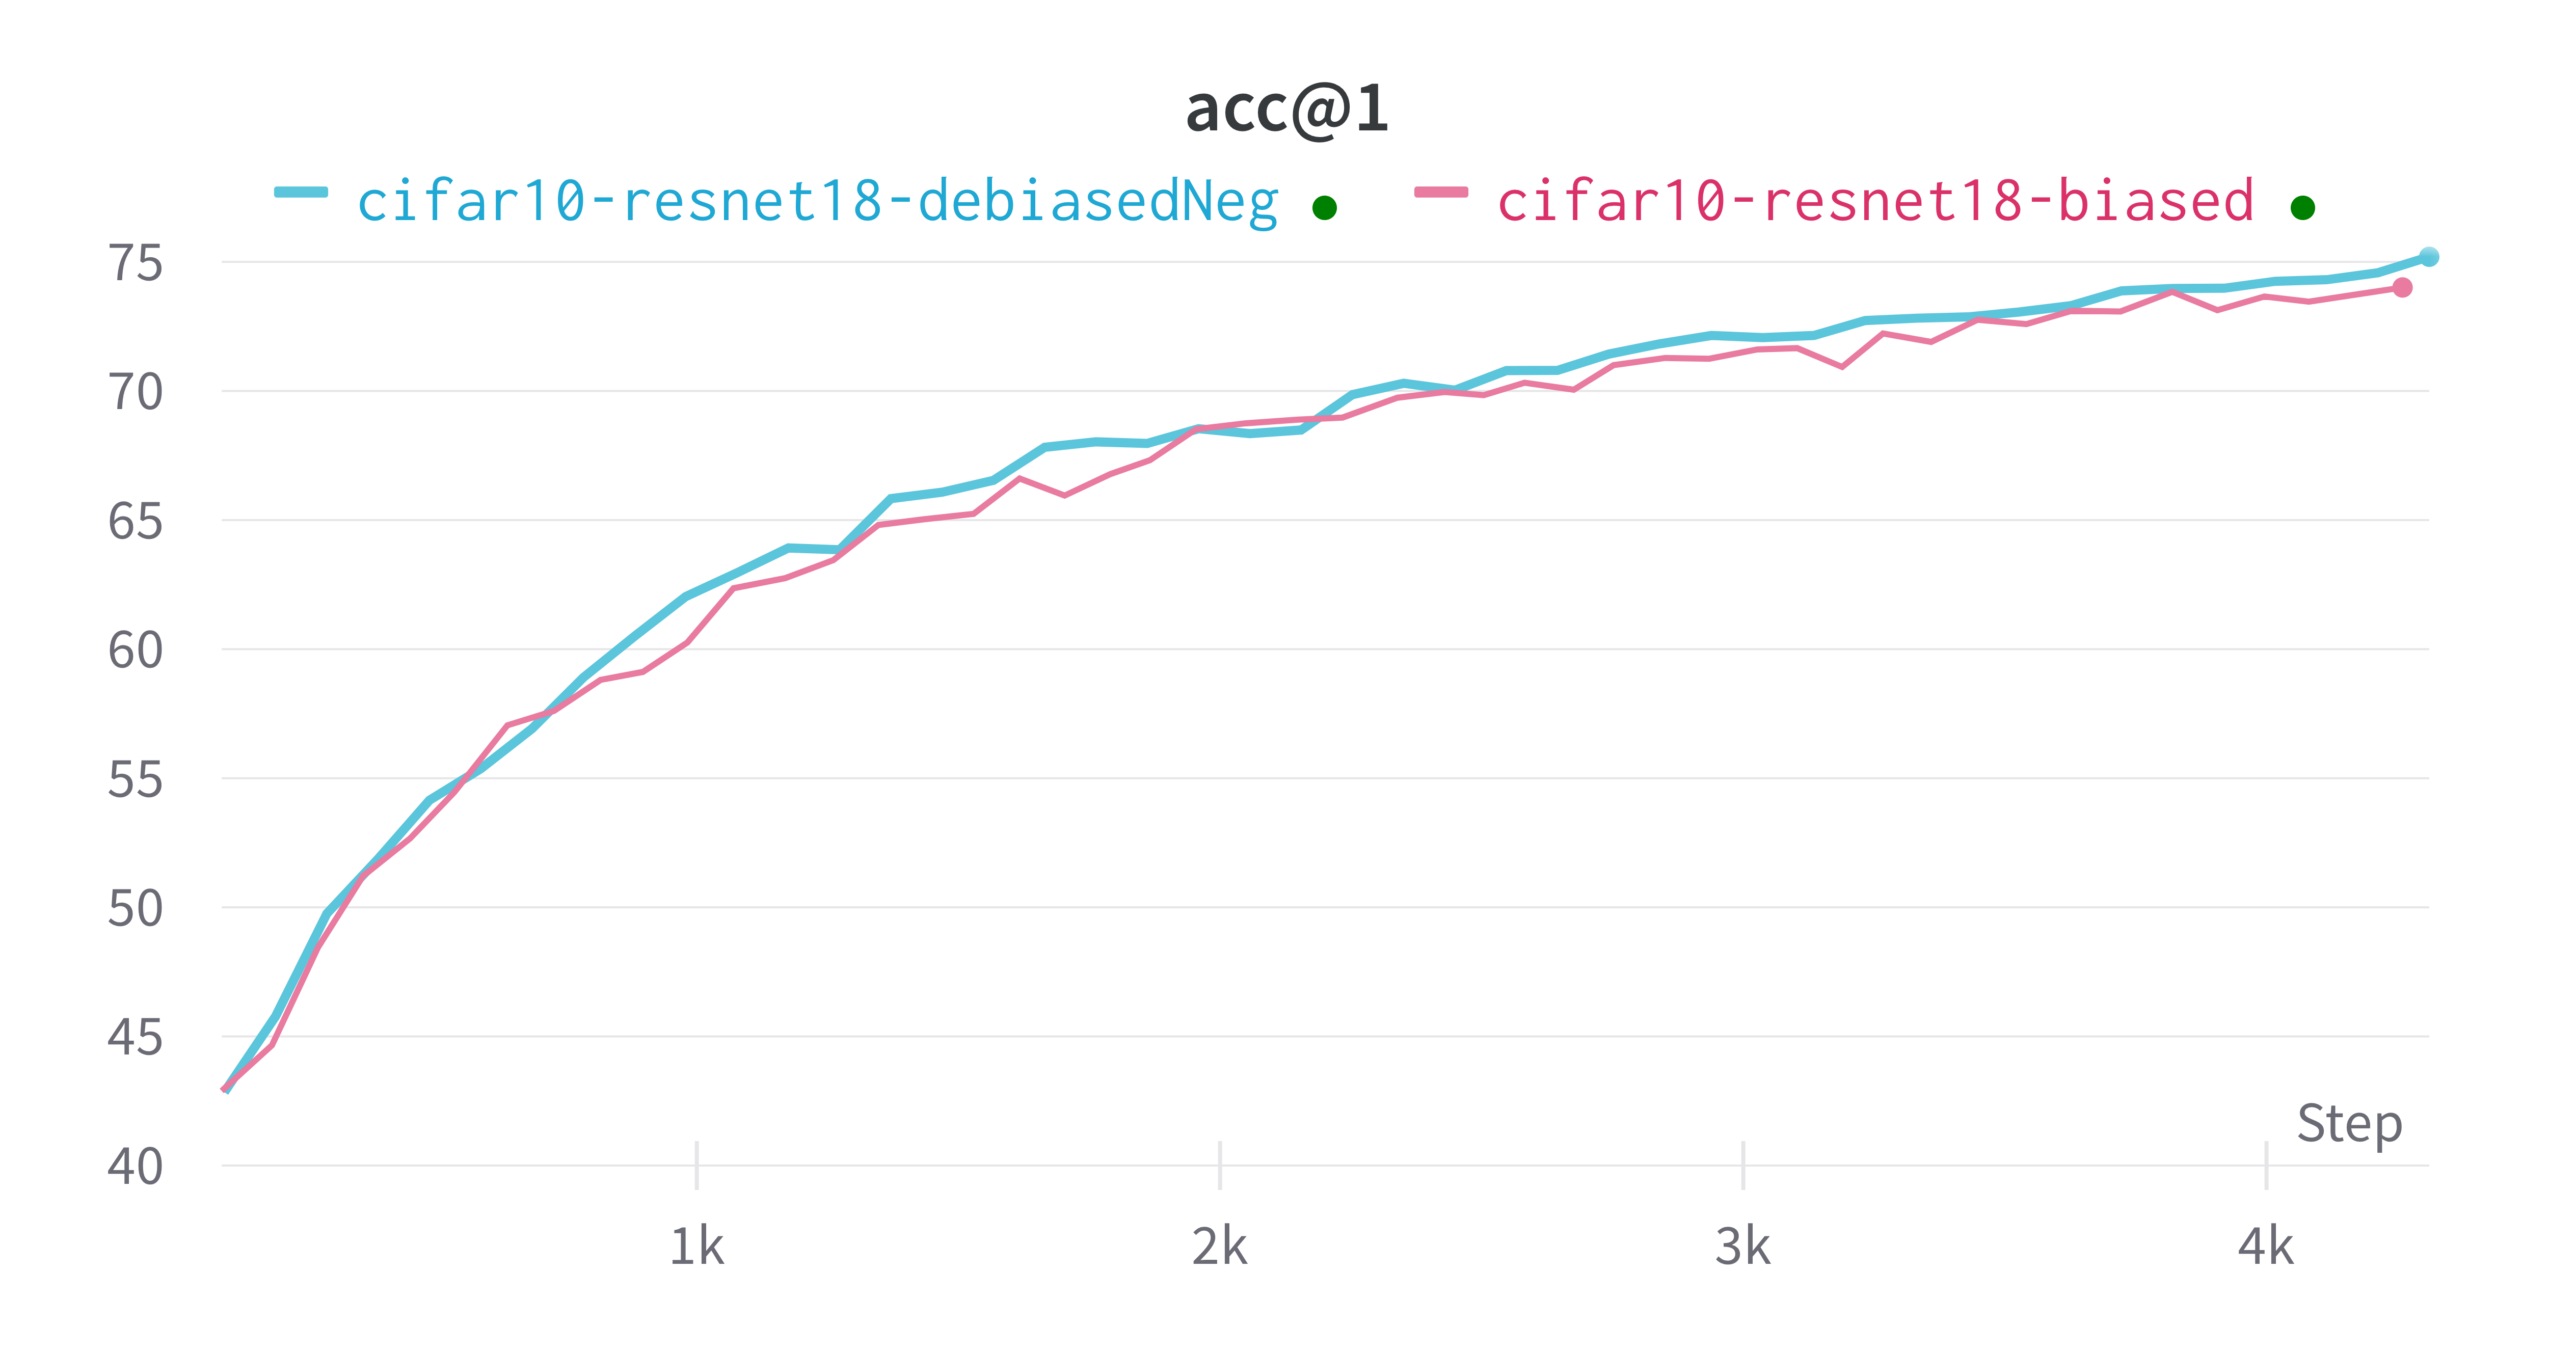
\includegraphics[width=\linewidth]{figures/baseline_acc1.png}
% \endminipage\hfill
% \minipage{0.49\textwidth}
% 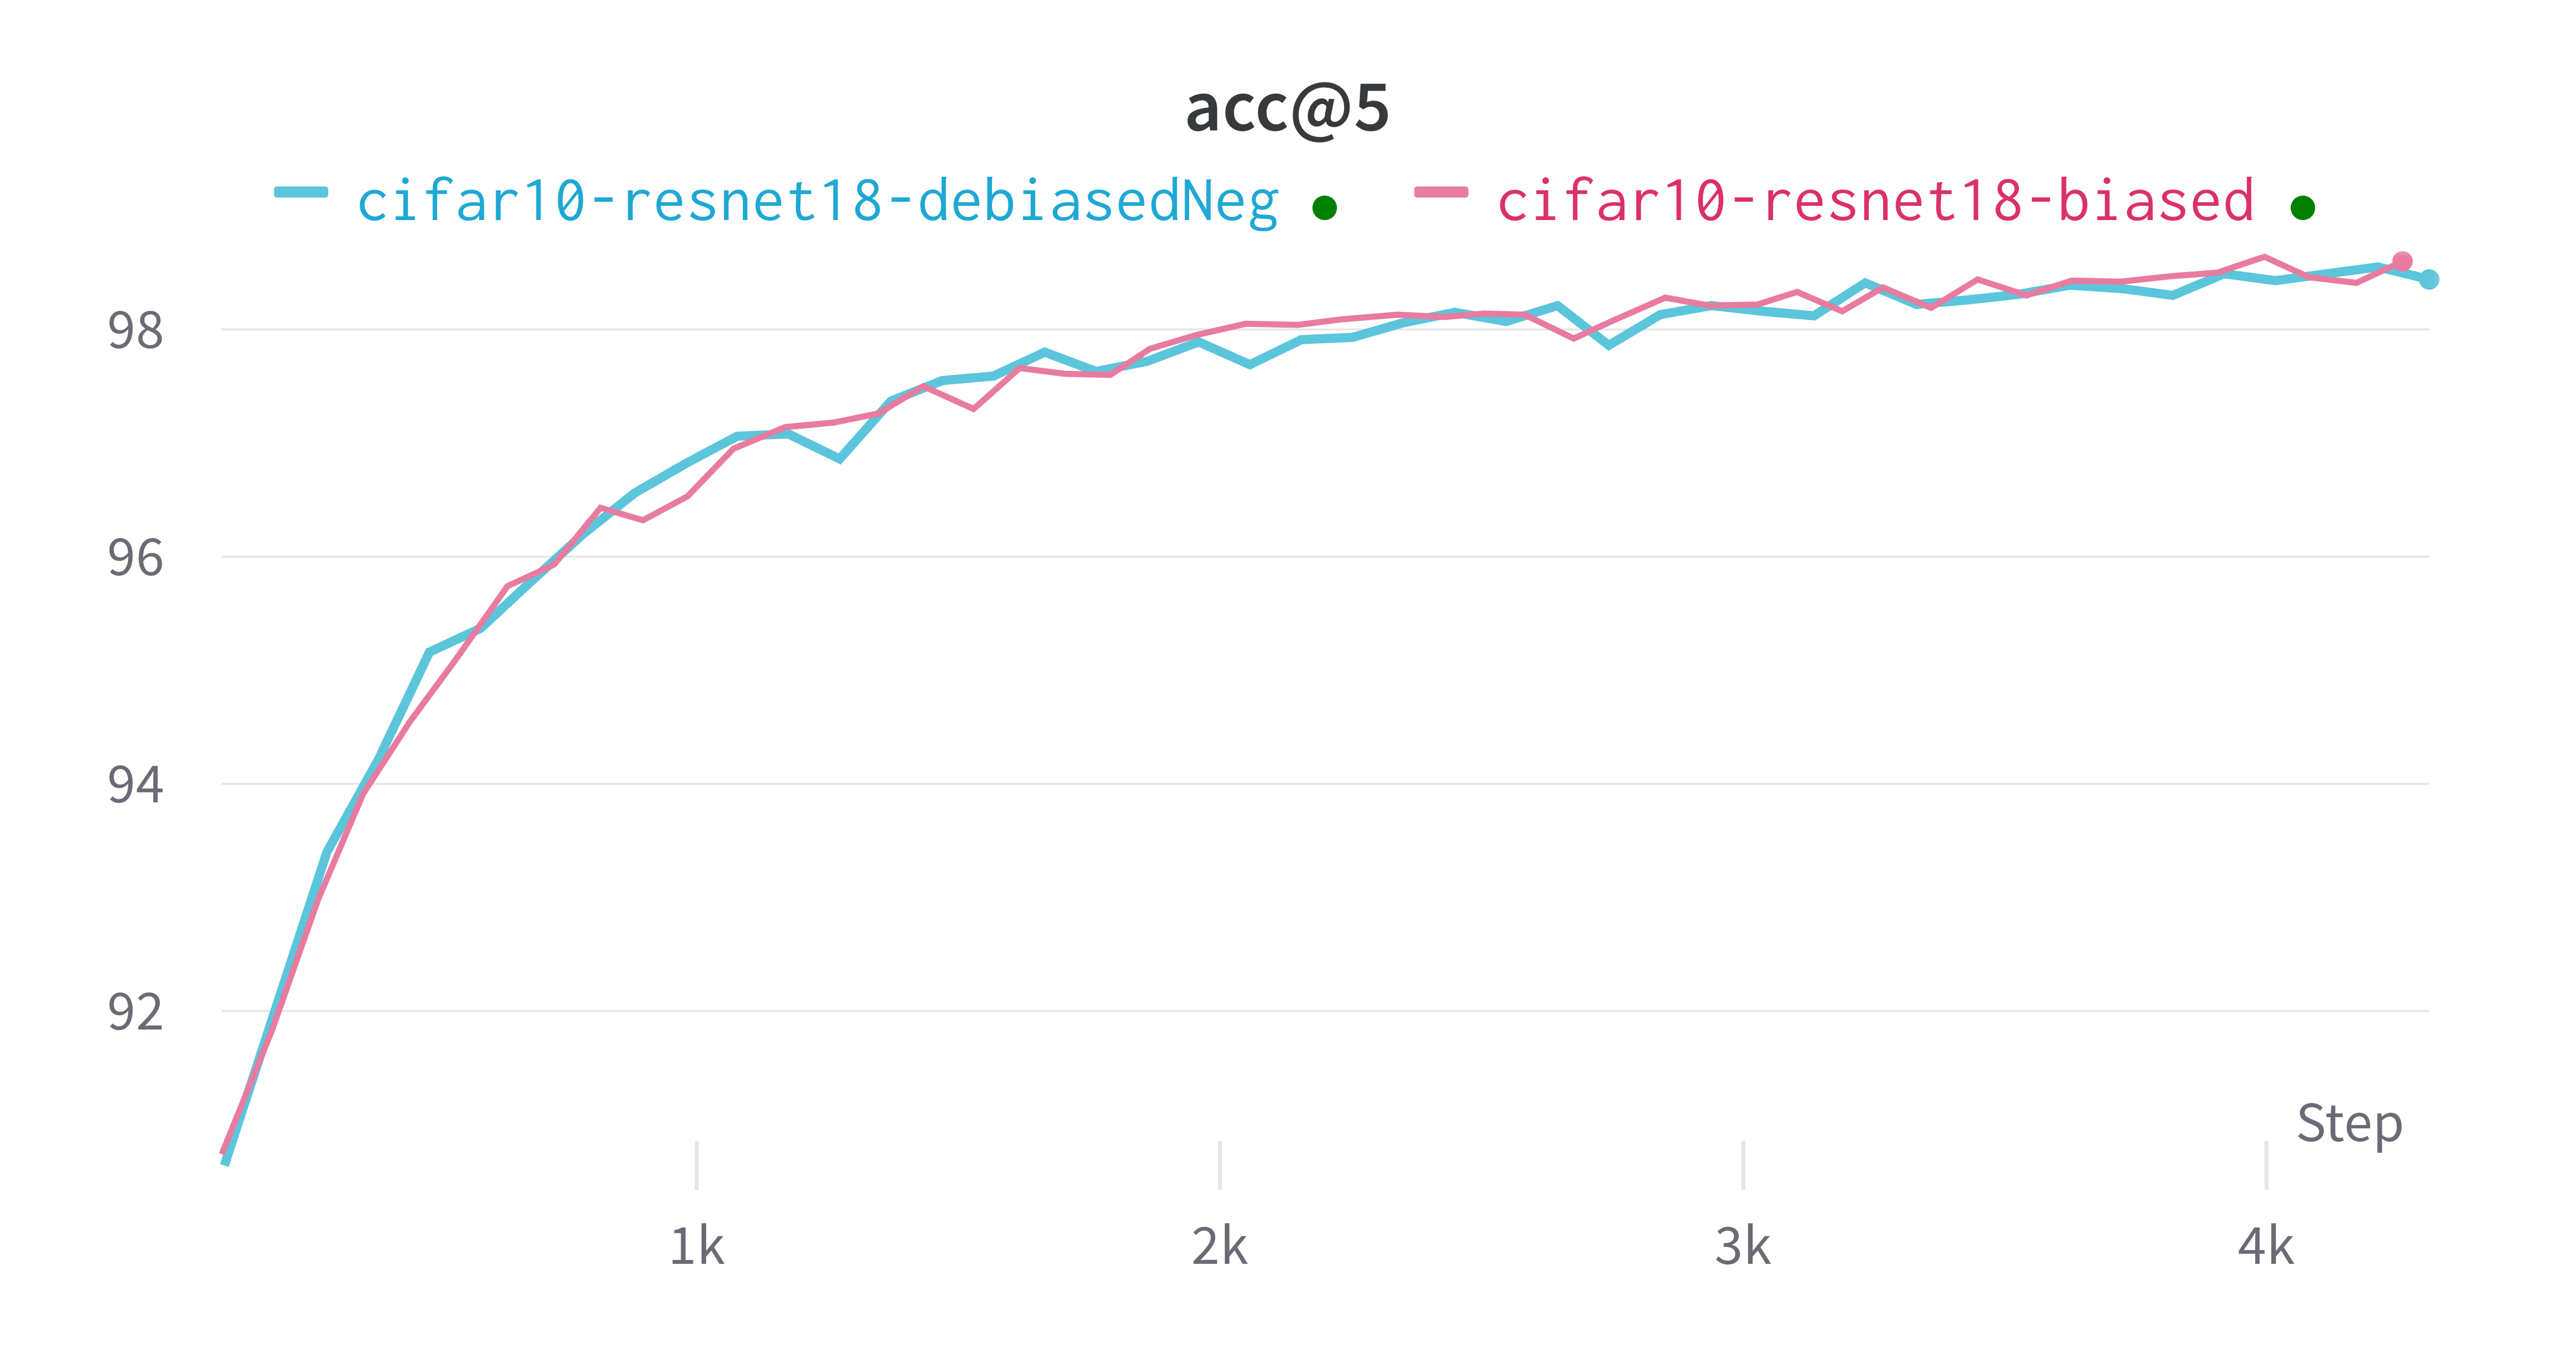
\includegraphics[width=\linewidth]{figures/baseline_acc5.png}
% \endminipage
% \caption{Classification accuracy on CIFAR10. Negative-Debiased loss is denoted as debiasedNeg.}
% \label{fig:fig1}
% \end{figure}

\subsection{Testing New Loss}
We run the same experiment for Positive-Debiased loss [\ref{eq:14}]. The code is available at our \href{https://github.com/intsystems/2023-Project-123}{GitHub}. Figure \ref{fig:fig2} shows a tangible difference between the performances of the novel loss and the previous losses. The accuracy advantage is prevalent from the very first steps of training both for Top-1 and Top-5 accuracy, meaning Positive-Debiased loss is more efficient in the early stages of training.

\begin{figure}[!htb]
\minipage{0.49\textwidth}
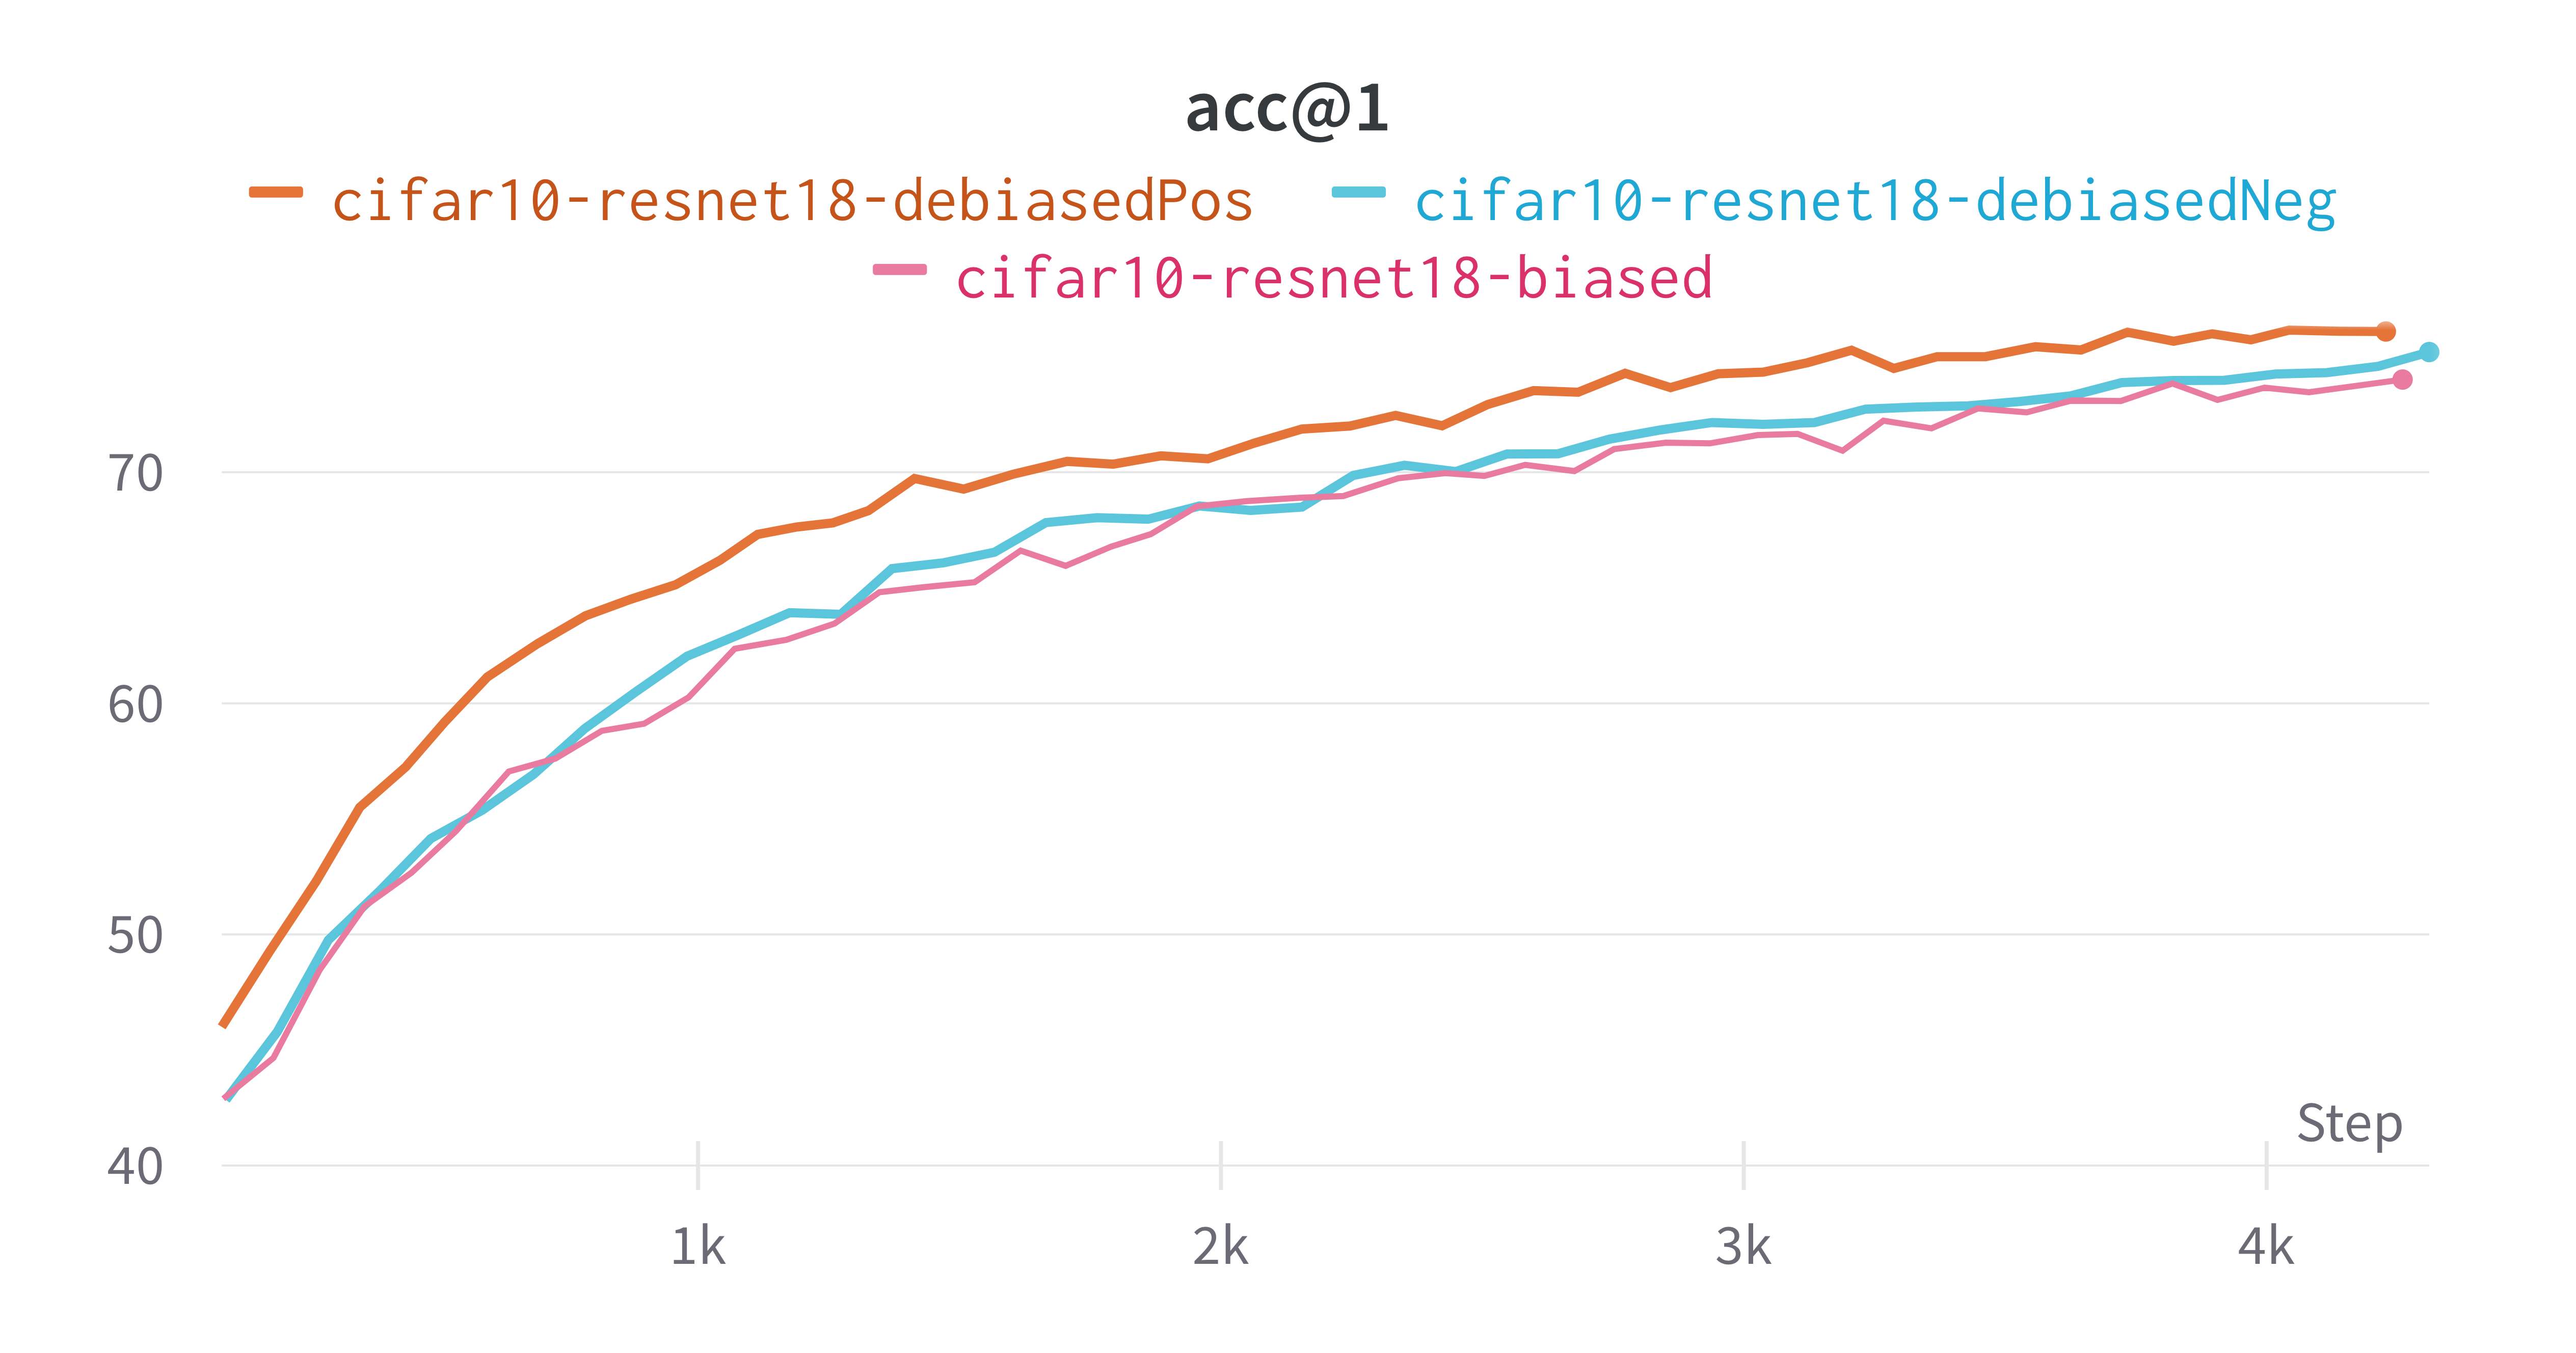
\includegraphics[width=\linewidth]{figures/3_losses.png}
\endminipage\hfill
\minipage{0.49\textwidth}
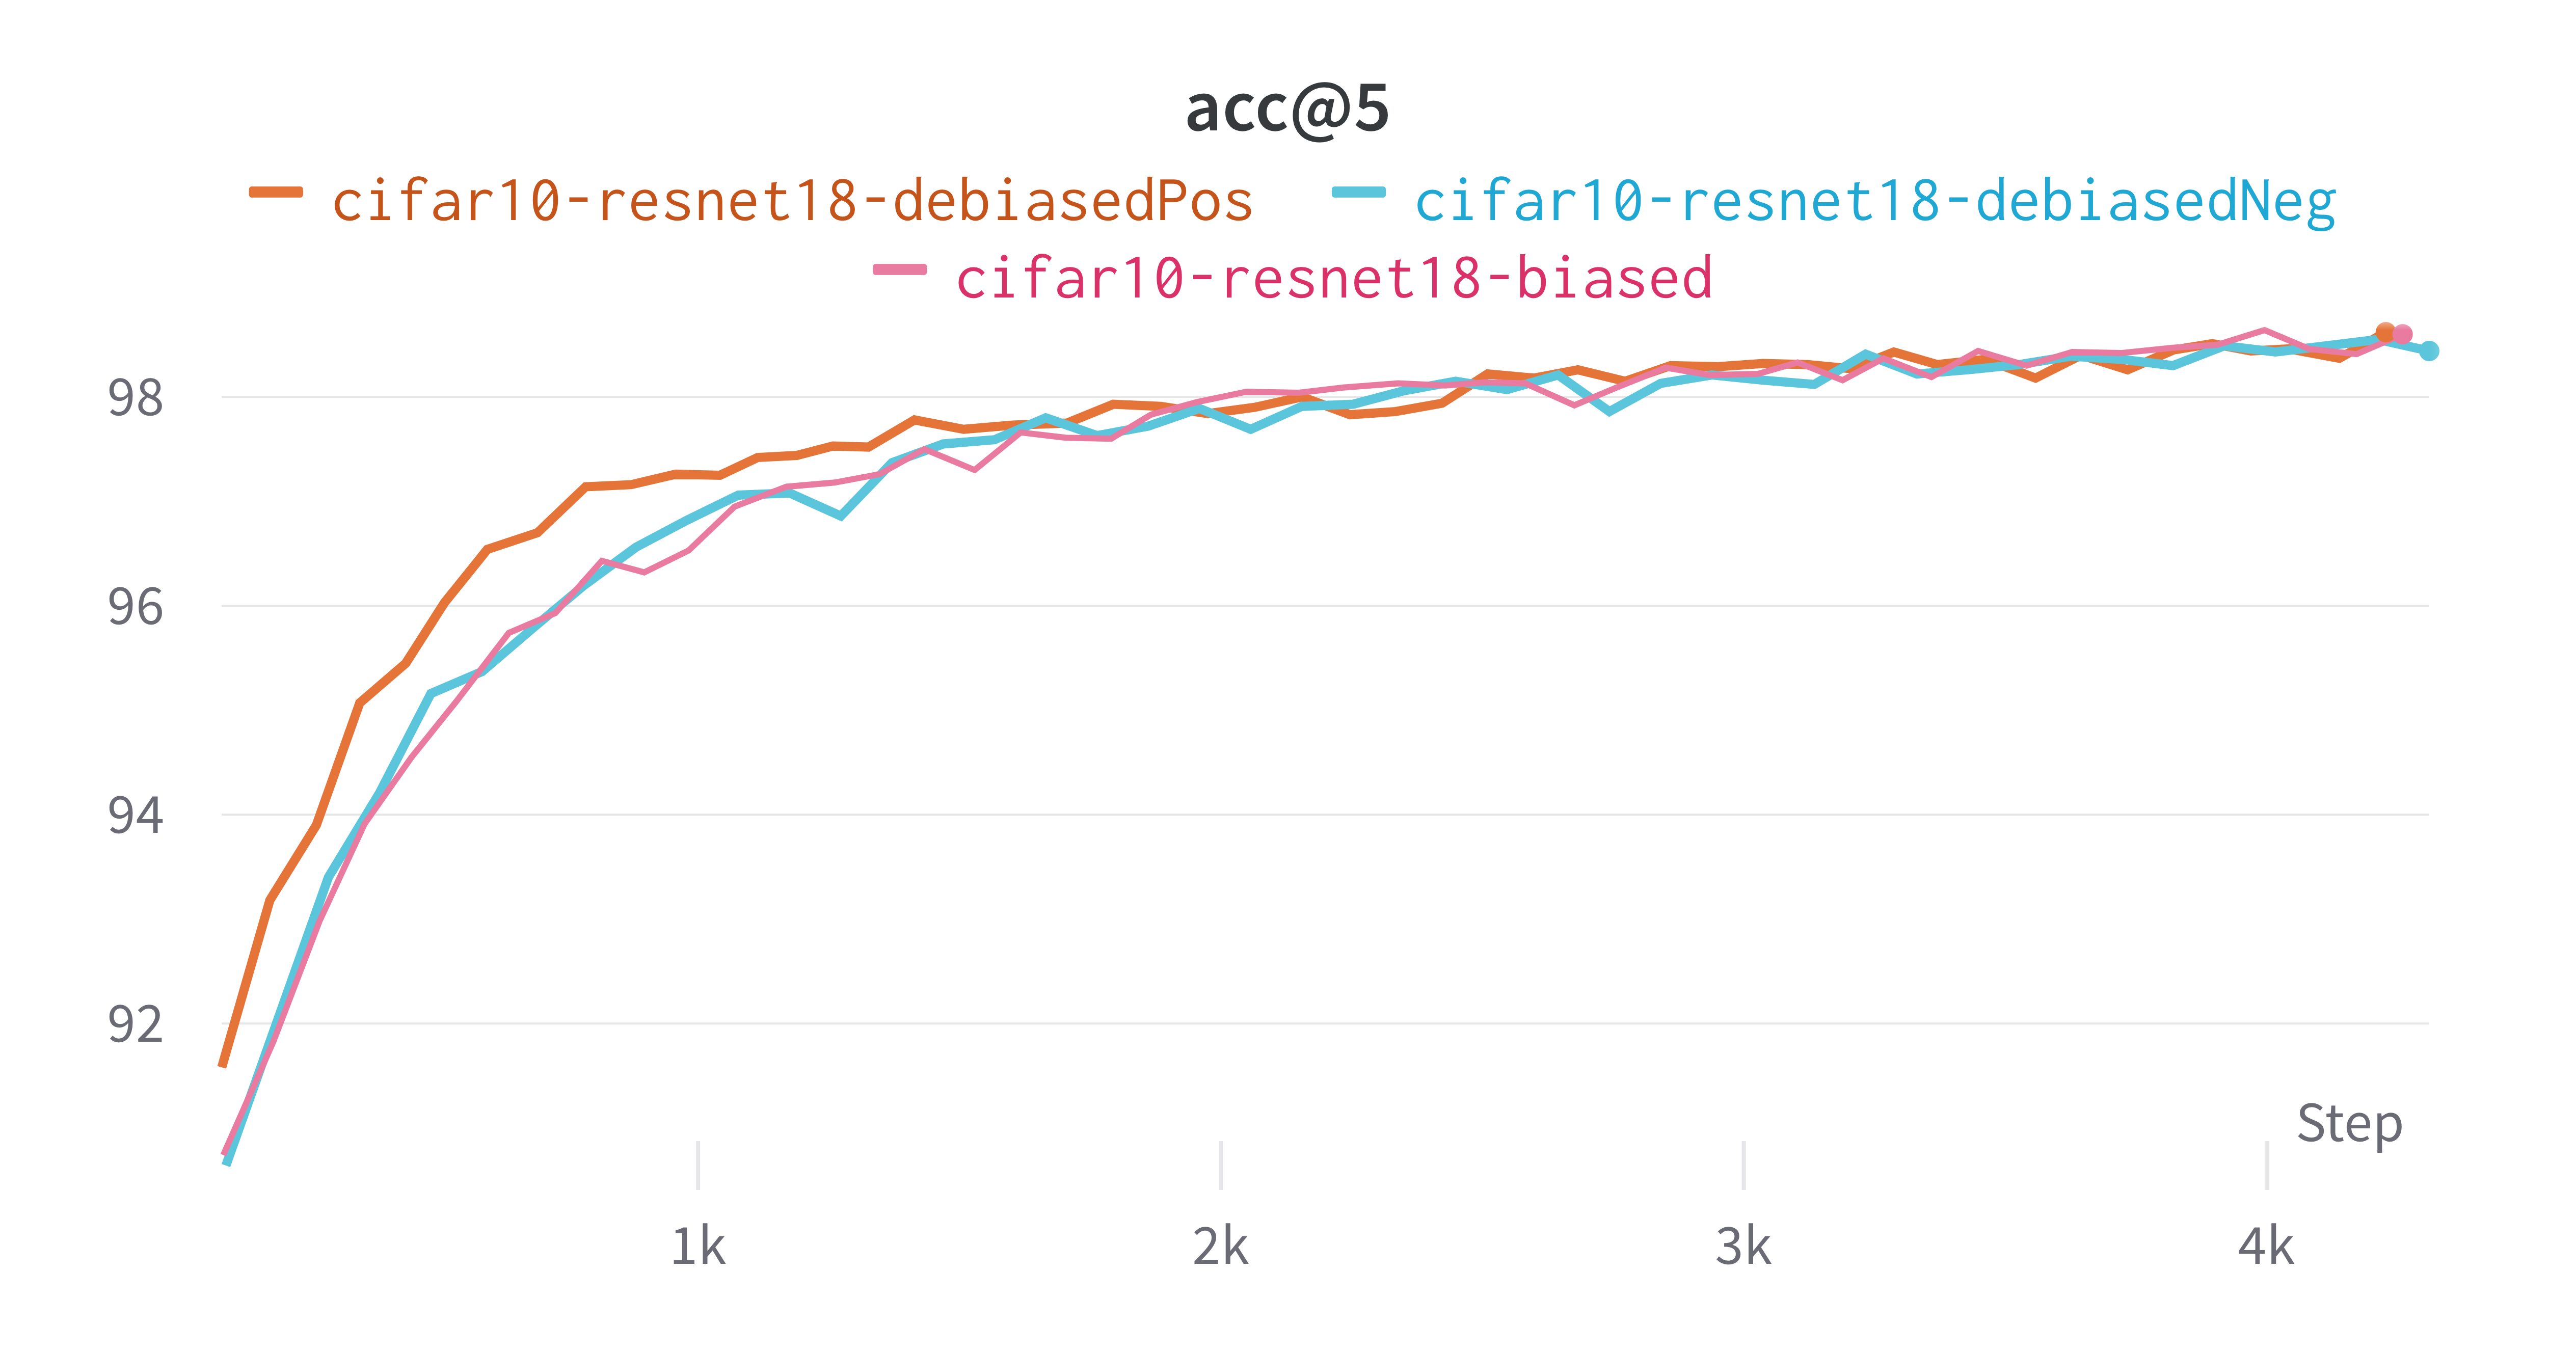
\includegraphics[width=\linewidth]{figures/3_losses_5.png}
\endminipage
\caption{Classification accuracy on CIFAR10, Negative- and Positive-Debiased losses are denoted as debiasedNeg and debiasedPos.}
\label{fig:fig2}
\end{figure}

To test the performance of the loss under the assumptions made in Section \ref{FP}, we artificially exclude False Negative errors via accessing ground truth labels during training, and discover that Positive-Debiased loss still outperforms Negative-Debiased loss [Figure \ref{fig:fig3}].

\begin{figure}
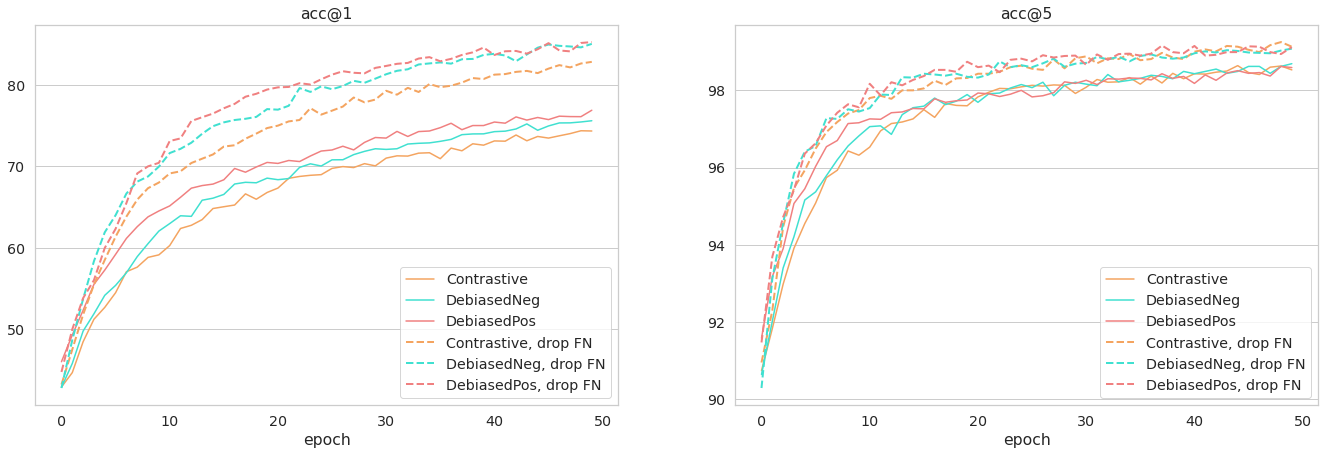
\includegraphics[width=1\textwidth]{figures/base_vs_dropfn.png}
\caption{Classification accuracy on CIFAR10 with dropping False Negatives}
\label{fig:fig3}
\end{figure}

To understand if Positive-Debiased loss is robust to noise, we apply Gaussian blur on train images with probability 0.3, and thus increase the False Positive rate. Figure \ref{fig:fig4} demonstrates that Positive-Debiased loss is able to mitigate False Positive errors significantly better than Negative-Debiased and Contrastive losses.

\begin{figure}
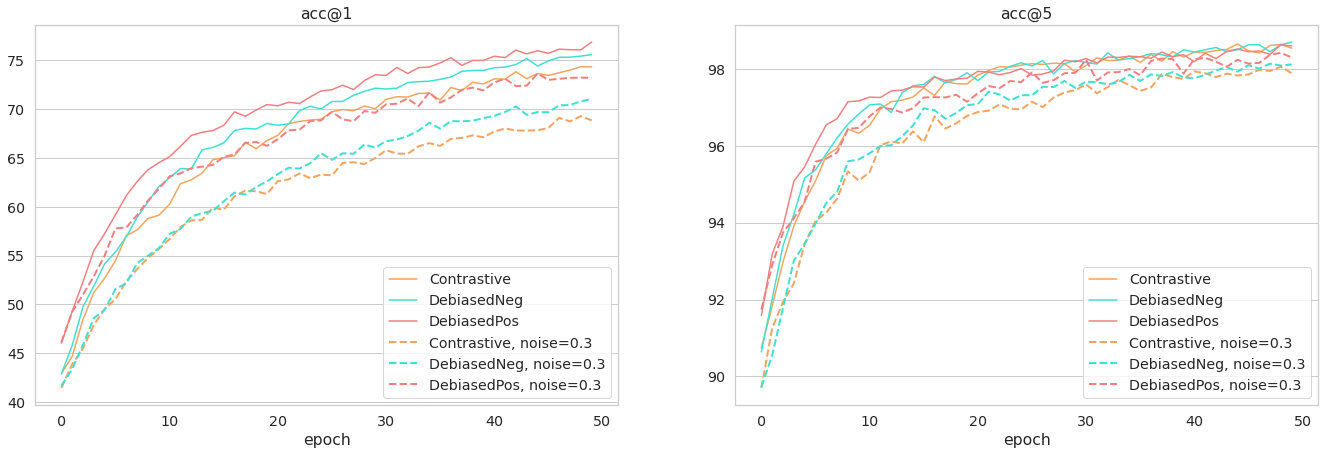
\includegraphics[width=1\textwidth]{figures/base_vs_noise.png}
\caption{Classification accuracy on CIFAR10 with an increased False Positive rate}
\label{fig:fig4}
\end{figure}

\begin{figure}
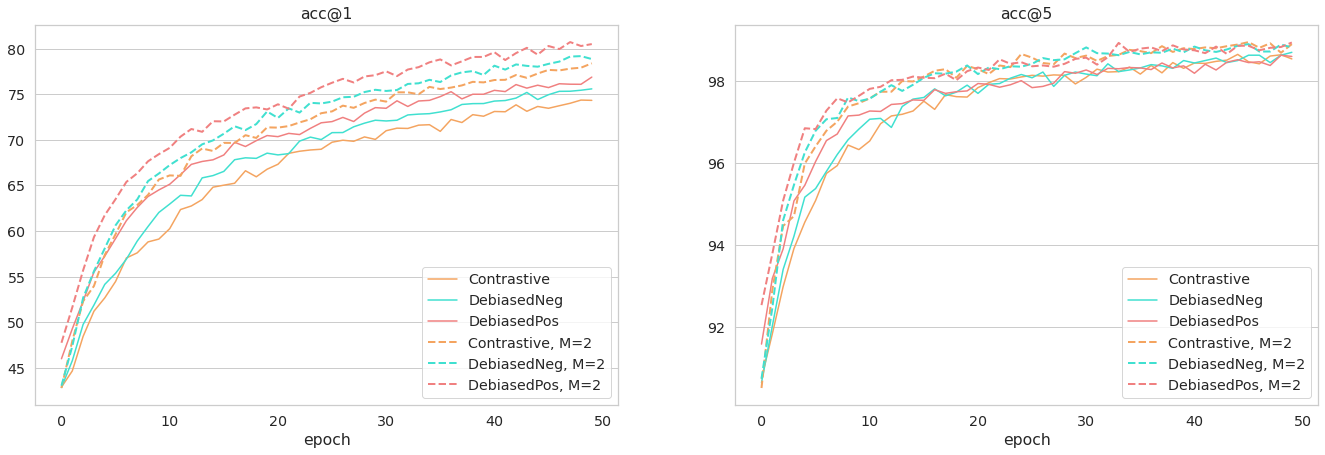
\includegraphics[width=1\textwidth]{figures/base_vs_M=2.png}
\caption{Classification accuracy on CIFAR10 with an increased positive sample size $M$}
\label{fig:fig5}
\end{figure}

Additionally, we test all three losses with increased positive sample size $M$ [Figure \ref{fig:fig5}]. Larger $M$ leads to better estimate of the loss both for Positive- and Negative-Debiased losses, yielding better accuracy as a result. It is worth noting that in all of the experiments Positive-Debiased loss achieves better accuracy in the earlier stages of training both for Top-1 and Top-5 scores.

\begin{figure}
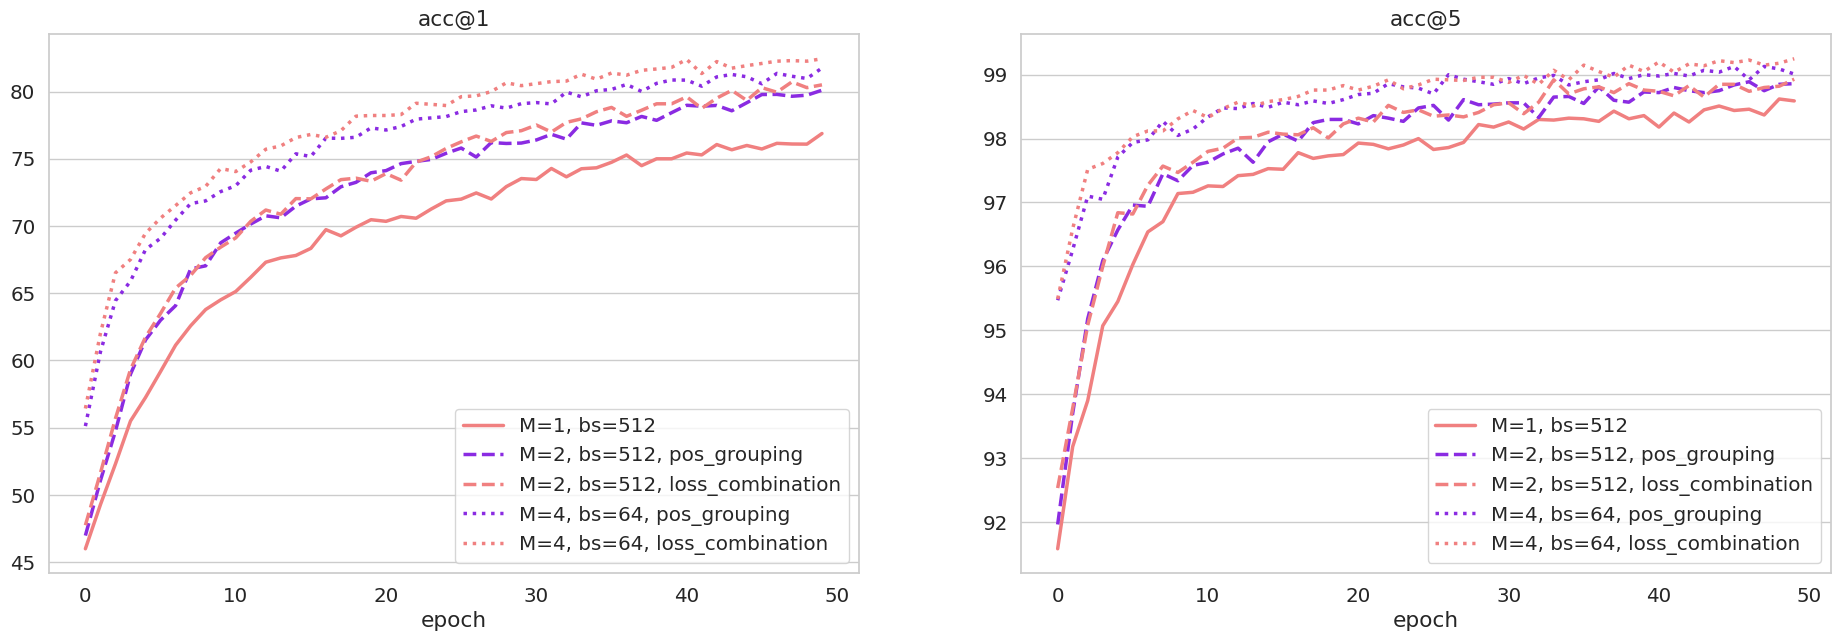
\includegraphics[width=1\textwidth]{figures/pg_vs_lc.png}
\caption{Classification accuracy on CIFAR10 with various positive sample aggregations}
\label{fig:fig6}
\end{figure}

\subsection{Positive Sample Aggregation} \label{pos_aggr}
In this experiment, we compare methods of aggregation over positive samples introduced in Section \ref{pos_aggr_theory}. We train SimCLR with the same parameters, except for setting batch size to 64 when testing $M=4$ for faster training. As expected, there is a trade-off between accuracy and speed. The results in Table \ref{tab:table} show that \textit{pos-grouping} improves over \textit{loss-combination} in accuracy, but is computationally slower. Figure \ref{fig:fig6} shows that with bigger $M$ the advantage of \textit{loss-combination} over \textit{pos-grouping} gets more significant. 

\begin{table}
    \caption{Aggregation over $M$ positive samples for DebiasedPos}
    \centering
    \begin{tabular}{llllll}
        \toprule
        Method  & $M$ & bs    & Training time (min)   & acc@1 & acc@5\\
        \midrule
        -   & 1 & 512   & 122.85    & 76.76 & 98.61\\
        \midrule
        pos-grouping    & 2 & 512   & \textbf{181.87}   & 80.1  & 98.86\\
        loss-combination    & 2 & 512   & 192.82    & \textbf{80.5} & \textbf{98.93}\\
        \midrule
        pos-grouping    & 4 & 64    & \textbf{278.88}   & 81.75 & 99.01\\
        loss-combination    & 4 & 64    & 308.25    & \textbf{82.44} & \textbf{99.25}\\
        \bottomrule
    \end{tabular}
    \label{tab:table}
\end{table}

\subsection{Discussion}
\begin{enumerate}
    \item Positive-Debiased loss is based on the assumption of true negative samples, i.e., with no False Negative errors; however, it still improves accuracy of classification when this assumption does not hold.
    \item Another implicit assumption we make is that the classes have uniform distribution, which is not true for many datasets, and it is an interesting direction of further research to additionally account for the biases in the class distribution.
\end{enumerate}

\section{Conclusion}
In this paper, we propose a new method for debiasing contrastive loss based on mitigating biases caused by False Positive errors. Theoretical analysis shows that computationally Positive-Debiased and baseline losses are equivalent. However, in a scenario with an increased False Positive rate our loss yields better accuracy, which shows that it is more robust. Moreover, Positive-Debiased loss is more dominant in the early epochs. We further explore 2 methods of aggregating loss over positive samples, and infer that \textit{pos-grouping} trains faster, while \textit{loss-combination} leads to better performance. 

% Interesting directions of future work include (1) trying the debiased objective in semi-supervised learning or few shot learning, and (2) studying the effect of how positive (similar) examples are drawn, e.g., analyzing different data augmentation techniques.

% \noindent\rule{16cm}{0.4pt}


\clearpage
\bibliographystyle{unsrtnat}
\bibliography{references}

\appendix
\newpage
\section{Proof of Theorem 2}
We recall \cref{thm:asympt}:

\asympt*

\begin{proof}
Let us denote:
\begin{flalign*}
    &P_{\text{est}} := \mathbb{E}_{\textbf{x}' \sim p} e^{f(\textbf{x})^Tf(\textbf{x}')}&\\
    &P_{\text{est}}^- := \mathbb{E}_{\textbf{x}^- \sim p_x^-} e^{f(\textbf{x})^Tf(\textbf{x}^-)}&\\
    &A_1 := -\log \frac{P_{\text{est}} - \tau^- P_{\text{est}}^-}{P_{\text{est}} + (N \tau^+ - \tau^-) P_{\text{est}}^-}&\\
    &A_2 := -\log \frac{P_{\text{est}} - \tau^- P_{\text{est}}^-}{P_{\text{est}} + (N \tau^+ - \tau^-) P_{\text{emp}}^-}&\\
    &A_3 := -\log \frac{P_{\text{est}} - \tau^- P_{\text{est}}^-}{P_{\text{emp}} + (N \tau^+ - \tau^-) P_{\text{emp}}^-}&\\
    &A_4 := -\log \frac{P_{\text{emp}} - \tau^- P_{\text{est}}^-}{P_{\text{emp}} + (N \tau^+ - \tau^-) P_{\text{emp}}^-}&\\
    &A_5 := -\log \frac{P_{\text{emp}} - \tau^- P_{\text{emp}}^-}{P_{\text{emp}} + (N \tau^+ - \tau^-) P_{\text{emp}}^-}
\end{flalign*}
Note that $e^{-1} \leq P_{\text{est}}, P_{\text{est}}^- \leq e$. We extend the proofs of Lemma A.2 and Theorem 3 from \citep{chuang2021debiased} to get results for DebiasedPos Loss.

\begin{enumerate}[leftmargin=*]
    \item
\begin{flalign*}
    &\Delta_1 := |A_2 - A_1| = \bigg| -\log \frac{P_{\text{est}} - \tau^- P_{\text{est}}^-}{P_{\text{est}} + (N \tau^+ - \tau^-) P_{\text{emp}}^-} + \log \frac{P_{\text{est}} - \tau^- P_{\text{est}}^-}{P_{\text{est}} + (N \tau^+ - \tau^-) P_{\text{est}}^-} \bigg|.&\\
    &\forall \varepsilon > 0: \mathbb{P} (\Delta_1 \geq \varepsilon) = \mathbb{P} \bigg(\bigg|\log \{P_{\text{est}} + (N \tau^+ - \tau^-) P_{\text{emp}}^-\} - \log \{P_{\text{est}} + (N \tau^+ - \tau^-) P_{\text{est}}^-\}\bigg| \geq \varepsilon \bigg) = &\\
    & = \mathbb{P} \bigg(\log \{P_{\text{est}} + (N \tau^+ - \tau^-) P_{\text{emp}}^-\} - \log \{P_{\text{est}} + (N \tau^+ - \tau^-) P_{\text{est}}^-\} \geq \varepsilon \bigg) + &\\
    & = \mathbb{P} \bigg(\log \{P_{\text{est}} + (N \tau^+ - \tau^-) P_{\text{emp}}^-\} - \log \{P_{\text{est}} + (N \tau^+ - \tau^-) P_{\text{est}}^-\} \leq -\varepsilon \bigg)
\end{flalign*}

The first term can be bounded as:
\begin{flalign*}
    &\mathbb{P} \bigg(\log \{P_{\text{est}} + (N \tau^+ - \tau^-) P_{\text{emp}}^-\} - \log \{P_{\text{est}} + (N \tau^+ - \tau^-) P_{\text{est}}^-\} \geq \varepsilon \bigg) =&\\
    &= \mathbb{P} \bigg(\log \frac{P_{\text{est}} + (N \tau^+ - \tau^-) P_{\text{emp}}^-}{P_{\text{est}} + (N \tau^+ - \tau^-) P_{\text{est}}^-} \geq \varepsilon \bigg)
        \leq
    \mathbb{P} \bigg(\frac{(N \tau^+ - \tau^-)(P_{\text{emp}}^- - P_{\text{est}}^-)}{P_{\text{est}} + (N \tau^+ - \tau^-) P_{\text{est}}^-} \geq \varepsilon \bigg)=&\\
    &= \mathbb{P} \bigg(P_{\text{emp}}^- - P_{\text{est}}^- \geq \varepsilon \bigg\{\frac{1}{N \tau^+ - \tau^-} P_{\text{est}} + P_{\text{est}}^- \bigg\}\bigg)
        \leq
    \mathbb{P} (P_{\text{emp}}^- - P_{\text{est}}^- \geq \varepsilon e^{-1})&\\
\end{flalign*}

Here we used the fact that $\log x \leq x - 1$ for $x > 0$, and $1/(N \tau^+ - \tau^-) P_{\text{est}} + P_{\text{est}}^- \geq e^{-1}$. Likewise bounding the second term:
$$\mathbb{P} \bigg(\log \{P_{\text{est}} + (N \tau^+ - \tau^-) P_{\text{emp}}^-\} - \log \{P_{\text{est}} + (N \tau^+ - \tau^-) P_{\text{est}}^-\} \leq -\varepsilon \bigg) \leq \mathbb{P} (P_{\text{est}}^- - P_{\text{emp}}^- \geq \varepsilon e^{-1})$$

and applying Hoeffding’s inequality, we have:
\begin{flalign*}
    &\mathbb{P} (\Delta_1 \geq \varepsilon) \leq \mathbb{P} (|P_{\text{emp}}^- - P_{\text{est}}^-| \geq \varepsilon e^{-1}) = \mathbb{P} \bigg(\bigg|\frac{1}{N} \sum \limits_{i=1}^N e^{f(\textbf{x})^T f(\textbf{u}_i)} - \mathbb{E}_{\textbf{x}^- \sim p_x^-} e^{f(\textbf{x})^Tf(\textbf{x}^-)}\bigg| \geq \varepsilon e^{-1}\bigg) \leq&\\
    &\leq 2 \exp\bigg(-\frac{2N \varepsilon^2 e^{-2}}{e - e^{-1}} \bigg) \leq 2 \exp\bigg(-\frac{2N \varepsilon^2}{e^3} \bigg) &\\
\end{flalign*}

Finally, we write the expectation of $\Delta_1$ as the integral of its tail probability
\begin{flalign*}
    &\big|\mathbb{E} A_2 - \mathbb{E} A_1 \big| \leq \mathbb{E} \Delta_1 \leq \int_0^\infty 2 \exp\bigg(-\frac{2N \varepsilon^2}{e^3} \bigg) d \varepsilon = \sqrt{\frac{\pi}{2N}} e^{3/2}.
\end{flalign*}

    \item
\begin{flalign*}
    &\Delta_2 := |A_3 - A_2| = \bigg| -\log \frac{P_{\text{est}} - \tau^- P_{\text{est}}^-}{P_{\text{emp}} + (N \tau^+ - \tau^-) P_{\text{emp}}^-} + \log \frac{P_{\text{est}} - \tau^- P_{\text{est}}^-}{P_{\text{est}} + (N \tau^+ - \tau^-) P_{\text{emp}}^-} \bigg|.&\\
    &\forall \varepsilon > 0: \mathbb{P} (\Delta_2 \geq \varepsilon) = \mathbb{P} \bigg(\bigg|\log \{P_{\text{emp}} + (N \tau^+ - \tau^-) P_{\text{emp}}^-\} - \log \{P_{\text{est}} + (N \tau^+ - \tau^-) P_{\text{emp}}^-\}\bigg| \geq \varepsilon \bigg)&\\
\end{flalign*}

We split the probability into a sum of two terms, and bound the first term as:
\begin{flalign*}
    &\mathbb{P} \bigg(\log \{P_{\text{emp}} + (N \tau^+ - \tau^-) P_{\text{emp}}^-\} - \log \{P_{\text{est}} + (N \tau^+ - \tau^-) P_{\text{emp}}^-\} \geq \varepsilon \bigg) =&\\
    &= \mathbb{P} \bigg(\log \frac{P_{\text{emp}} + (N \tau^+ - \tau^-) P_{\text{emp}}^-}{P_{\text{est}} + (N \tau^+ - \tau^-) P_{\text{emp}}^-} \geq \varepsilon \bigg)
        \leq
    \mathbb{P} \bigg(\frac{P_{\text{emp}} - P_{\text{est}}}{P_{\text{est}} + (N \tau^+ - \tau^-) P_{\text{emp}}^-} \geq \varepsilon \bigg)=&\\
    &= \mathbb{P} \bigg(P_{\text{emp}} - P_{\text{est}} \geq \varepsilon \big\{P_{\text{est}} + (N \tau^+ - \tau^-) P_{\text{emp}}^-\big\}\bigg)
        \leq
    \mathbb{P} (P_{\text{emp}} - P_{\text{est}} \geq \varepsilon e^{-1})&\\
\end{flalign*}

This holds because with $N$ large enough, $N \tau^+ \geq \tau^-$, and thus $1/(N \tau^+ - \tau^-) P_{\text{est}} + P_{\text{est}}^- \geq e^{-1}$.
\begin{flalign*}
    &\mathbb{P} (\Delta_2 \geq \varepsilon) \leq \mathbb{P} (|P_{\text{emp}} - P_{\text{est}}| \geq \varepsilon e^{-1}) = &\\
    &= \mathbb{P} \bigg(\bigg| \frac{1}{N+2} \bigg(\sum \limits_{i=1}^N e^{f(\textbf{x})^T f(\textbf{u}_i)} + e^{f(\textbf{x})^T f(\textbf{v})} + e^{f(\textbf{x})^T f(\textbf{x})}\bigg) - \mathbb{E}_{\textbf{x}' \sim p} e^{f(\textbf{x})^Tf(\textbf{x}')} \bigg| \geq \varepsilon e^{-1}\bigg) \leq&\\
    &\leq 2 \exp\bigg(-\frac{2(N+2) \varepsilon^2}{e^3} \bigg) &\\
    &\big|\mathbb{E} A_3 - \mathbb{E} A_2 \big| \leq \mathbb{E} \Delta_2 \leq \int_0^\infty 2 \exp\bigg(-\frac{2(N+2) \varepsilon^2}{e^3} \bigg) d \varepsilon = \sqrt{\frac{\pi}{2(N+2)}} e^{3/2}.
\end{flalign*}

    \item
\begin{flalign*}
    &\Delta_3 := |A_3 - A_4| = \bigg| -\log \frac{P_{\text{est}} - \tau^- P_{\text{est}}^-}{P_{\text{emp}} + (N \tau^+ - \tau^-) P_{\text{emp}}^-} + \log \frac{P_{\text{emp}} - \tau^- P_{\text{est}}^-}{P_{\text{emp}} + (N \tau^+ - \tau^-) P_{\text{emp}}^-}\bigg|.&\\
    &\forall \varepsilon > 0: \mathbb{P} (\Delta_3 \geq \varepsilon) = \mathbb{P} \bigg(\bigg|\log \{P_{\text{emp}} - \tau^- P_{\text{est}}^-\} - \log \{P_{\text{est}} - \tau^- P_{\text{est}}^-\}\bigg| \geq \varepsilon \bigg)&\\
\end{flalign*}

We split the probability into a sum of two terms, and bound the first term as:
\begin{flalign*}
    &\mathbb{P} \bigg(\log \{P_{\text{emp}} - \tau^- P_{\text{est}}^-\} - \log \{P_{\text{est}} - \tau^- P_{\text{est}}^-\} \geq \varepsilon \bigg) =&\\
    &= \mathbb{P} \bigg(\log \frac{P_{\text{emp}} - \tau^- P_{\text{est}}^-}{P_{\text{est}} - \tau^- P_{\text{est}}^-} \geq \varepsilon \bigg)
        \leq
    \mathbb{P} \bigg(\frac{P_{\text{emp}} - P_{\text{est}}}{P_{\text{est}} - \tau^- P_{\text{est}}^-} \geq \varepsilon \bigg)=&\\
    &= \mathbb{P} \bigg(P_{\text{emp}} - P_{\text{est}} \geq \varepsilon \big\{P_{\text{est}} - \tau^-P_{\text{est}}^-\big\}\bigg)
        \leq
    \mathbb{P} (P_{\text{emp}} - P_{\text{est}} \geq \varepsilon \tau^+ e^{-1})&\\
\end{flalign*}

This time the bound is different because $P_{\text{est}} - \tau^-P_{\text{est}}^- = \tau^+ P_{\text{est}}^+ := \tau^+ \mathbb{E}_{\textbf{x}^+ \sim p_x^+} e^{f(\textbf{x})^Tf(\textbf{x}^+)} \geq \tau^+ e^{-1}$.
\begin{flalign*}
    &\mathbb{P} (\Delta_3 \geq \varepsilon) \leq \mathbb{P} (|P_{\text{emp}} - P_{\text{est}}| \geq \varepsilon \tau^+ e^{-1}) = &\\
    &= \mathbb{P} \bigg(\bigg| \frac{1}{N+2} \bigg(\sum \limits_{i=1}^N e^{f(\textbf{x})^T f(\textbf{u}_i)} + e^{f(\textbf{x})^T f(\textbf{v})} + e^{f(\textbf{x})^T f(\textbf{x})}\bigg) - \mathbb{E}_{\textbf{x}' \sim p} e^{f(\textbf{x})^Tf(\textbf{x}')} \bigg| \geq \varepsilon \tau^+ e^{-1}\bigg) \leq&\\
    &\leq 2 \exp\bigg(-\frac{2(N+2) \varepsilon^2 (\tau^+)^2}{e^3} \bigg) &\\
    &\big|\mathbb{E} A_3 - \mathbb{E} A_4 \big| \leq \mathbb{E} \Delta_3 \leq \int_0^\infty 2 \exp\bigg(-\frac{2(N+2) \varepsilon^2 (\tau^+)^2}{e^3} \bigg) d \varepsilon = \frac{1}{\tau^+} \sqrt{\frac{\pi}{2(N+2)}} e^{3/2}.
\end{flalign*}

    \item
\begin{flalign*}
    &\Delta_4 := |A_5 - A_4| = \bigg| -\log \frac{P_{\text{emp}} - \tau^- P_{\text{emp}}^-}{P_{\text{emp}} + (N \tau^+ - \tau^-) P_{\text{emp}}^-} + \log \frac{P_{\text{emp}} - \tau^- P_{\text{est}}^-}{P_{\text{emp}} + (N \tau^+ - \tau^-) P_{\text{emp}}^-} \bigg|.&\\
    &\forall \varepsilon > 0: \mathbb{P} (\Delta_4 \geq \varepsilon) = \mathbb{P} \bigg(\bigg|\log \{P_{\text{emp}} - \tau^- P_{\text{est}}^-\} - \log \{P_{\text{emp}} - \tau^- P_{\text{emp}}^-\}\bigg| \geq \varepsilon \bigg)&\\
\end{flalign*}

We split the probability into a sum of two terms, and bound the first term as:
\begin{flalign*}
    &\mathbb{P} \bigg(\log \{P_{\text{emp}} - \tau^- P_{\text{est}}^-\} - \log \{P_{\text{emp}} - \tau^- P_{\text{emp}}^-\} \geq \varepsilon \bigg) =&\\
    &= \mathbb{P} \bigg(\log \frac{P_{\text{emp}} - \tau^- P_{\text{est}}^-}{P_{\text{emp}} - \tau^- P_{\text{emp}}^-} \geq \varepsilon \bigg)
        \leq
    \mathbb{P} \bigg(\frac{\tau^-(P_{\text{emp}}^- - P_{\text{est}}^-)}{P_{\text{emp}} - \tau^- P_{\text{emp}}^-} \geq \varepsilon \bigg)=&\\
    &= \mathbb{P} \bigg(P_{\text{emp}}^- - P_{\text{est}}^- \geq \varepsilon \bigg\{\frac{1}{\tau^-} P_{\text{emp}} - P_{\text{emp}}^-\bigg\}\bigg)
        \leq
    \mathbb{P} \bigg(P_{\text{emp}}^- - P_{\text{est}}^- \geq \varepsilon \bigg( \frac{\tau^+}{\tau^-} e^{-1} - \delta\bigg)\bigg)&\\
\end{flalign*}

To get a lower bound of the expression in braces for a large $N$, we will take a slightly smaller value than its limit.
\begin{flalign*}
    &\frac{1}{\tau^-} P_{\text{emp}} - P_{\text{emp}}^- = \frac{1}{\tau^-} \frac{1}{N+2} \bigg(\sum \limits_{i=1}^N e^{f(\textbf{x})^T f(\textbf{u}_i)} + e^{f(\textbf{x})^T f(\textbf{v})} + e^{f(\textbf{x})^T f(\textbf{x})}\bigg) - \frac{1}{N} \sum \limits_{i=1}^N e^{f(\textbf{x})^T f(\textbf{u}_i)} =&\\
    &= \bigg(\frac{1}{\tau^-}\frac{1}{N+2} - \frac{1}{N}\bigg)\bigg(\sum \limits_{i=1}^N e^{f(\textbf{x})^T f(\textbf{u}_i)}\bigg) + \frac{e^{f(\textbf{x})^T f(\textbf{v})} + e^{f(\textbf{x})^T f(\textbf{x})}}{\tau^-(N+2)} \xrightarrow[N \to \infty]{} \frac{e^{-1}}{\tau^-} - e^{-1} = \frac{\tau^+}{\tau^-} e^{-1}&\\
\end{flalign*}

\begin{flalign*}
    &\mathbb{P} (\Delta_4 \geq \varepsilon) \leq \mathbb{P} \bigg(|P_{\text{emp}}^- - P_{\text{est}}^-| \geq \varepsilon \bigg( \frac{\tau^+}{\tau^-} e^{-1} - \delta\bigg)\bigg) = &\\
    &= \mathbb{P} \bigg(\bigg| \frac{1}{N} \sum \limits_{i=1}^N e^{f(\textbf{x})^T f(\textbf{u}_i)} - \mathbb{E}_{\textbf{x}^- \sim p_x^-} e^{f(\textbf{x})^Tf(\textbf{x}^-)} \bigg| \geq \varepsilon \bigg( \frac{\tau^+}{\tau^-} e^{-1} - \delta\bigg)\bigg) \leq&\\
    &\leq 2 \exp\bigg(-\frac{2N \varepsilon^2 ( (\tau^+/ \tau^-) e^{-1} - \delta)^2}{e} \bigg) =: 2 \exp\bigg(-\frac{2N \varepsilon^2 ( \tau^+/\tau^- - \delta)^2}{e^3} \bigg)&\\
    &\big|\mathbb{E} A_5 - \mathbb{E} A_4 \big| \leq \mathbb{E} \Delta_4 \leq \int_0^\infty 2 \exp\bigg(-\frac{2N \varepsilon^2 ( \tau^+/\tau^- - \delta)^2}{e^3} \bigg) d \varepsilon =&\\
    &= \frac{1}{\tau^+/ \tau^- - \delta} \sqrt{\frac{\pi}{2N}} e^{3/2} =: \bigg(\frac{\tau^-}{\tau^+} - \delta\bigg) \sqrt{\frac{\pi}{2N}} e^{3/2}.&\\
\end{flalign*}

\end{enumerate}

The result follows by summing all four absolute differences:
\begin{flalign*}
    &\big|\tilde{L}_{\text{DebiasedPos}}^N (f) - L_{\text{DebiasedPos}}^N (f)\big| = \big|\mathbb{E} A_1 - \mathbb{E} A_5\big| \leq \big|\mathbb{E} A_1 - \mathbb{E} A_2\big| + \big|\mathbb{E} A_2 - \mathbb{E} A_3\big| + \big|\mathbb{E} A_3 - \mathbb{E} A_4\big| + \big|\mathbb{E} A_4 - \mathbb{E} A_5\big| \leq&\\
    &\leq \bigg[\bigg(1 + \frac{\tau^-}{\tau^+} + \delta\bigg) \sqrt{\frac{\pi}{2N}} + \bigg(1 + \frac{1}{\tau^+}\bigg) \sqrt{\frac{\pi}{2(N + 2)}}\bigg] e^{3/2}&\\
\end{flalign*}

\end{proof}

\end{document}